\documentclass[a4paper,12pt,french]{book}
\usepackage[margin=2cm]{geometry}
\usepackage[thinfonts]{uglix2}
\nouveaustyle

\begin{document}
\titre{Files - projet}{NSI2}{2020} 



Une grande surface possède n caisses. On choisit une unité de temps arbitraire (le tour) et on décide que lorsqu'un client passe à la caisse, cela prend un temps aléatoire compris entre 1 et n unités de temps.\\
À chaque unité de temps, un client arrive aux caisses.\\
On commence la simulation avec n clients qui arrivent.\\
On aimerait simuler le temps d'attente aux caisses et évaluer le temps d'attente moyen par client.\\


\section*{Avec une seule file}

On décide qu'une seule file existe : les clients attendent dans la file et dès qu'une caisse se libère, le premier client dans la file est reçu.

\subsection*{Simulation}
 Voici un début de simulation avec n=3 caisses
\subsubsection*{Initialisation}
\double
{
L'heure est \texttt{00}.\\
Puisqu'il y a 3 caisses, on place 3 clients dans la file (les carrés verts).
Pour l'instant personne n'a attendu donc le total des temps d'attente est \texttt{00}.\\
Les trois caisses sont libres : elles sont bleues, avec un temps d'attente de zéro.
}
{
    \fbox{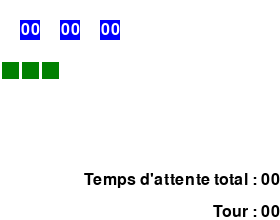
\includegraphics[width=4cm]{img/single_queue00}}
}{4cm}


\subsubsection*{Première itération}
\double
{
L'horloge a fait un tour.\\
Les 3 clients sont passés en caisse : les deux dernières prendront 3 tours pour traiter les achats de son client, la première 2 tours.\\
Un nouveau client se présente et attend.

}
{
    \fbox{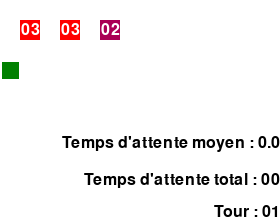
\includegraphics[width=4cm]{img/single_queue01}}
}{4cm}


\subsubsection*{Deuxième itération}
\double 
{
L'horloge a fait un tour.\\
Un nouveau client arrive dans la file.\\
Il est obligé d'attendre lui aussi.
Pour l'instant le temps d'attente total n'est pas actualisé : on attend qu'un client soit servi avant de comptabiliser son temps d'attente.
}
{
    \fbox{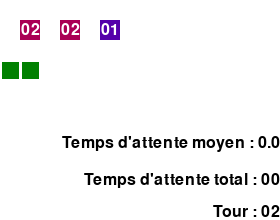
\includegraphics[width=4cm]{img/single_queue02}}
}{4cm}

\subsubsection*{Troisième itération}
\double
{
L'horloge a fait un tour.\\
Le client qui attendait depuis 2 tours est reçu, on actualise le temps d'attente total.
Il passe dans la première caisse.
Au total, 4 clients ont été reçus, avec un temps d'attente total de 2 tours, donc un temps d'attente moyen de 0.5 tour par client.\\
Un nouveau client se présente dans la file.\\
}
{
    \fbox{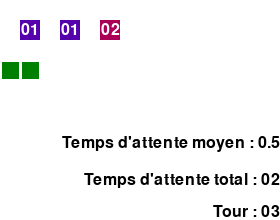
\includegraphics[width=4cm]{img/single_queue03}}
}{4cm}

\subsubsection*{Quatrième itération}
\double
{
L'horloge a fait un tour.\\
Les 2 clients précédents sont servis, on ajoute leurs temps d'attente, un nouveau client arrive, \textit{et c\ae tera}.
}
{
    \fbox{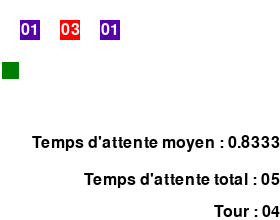
\includegraphics[width=4cm]{img/single_queue04}}
}{4cm}

\subsection*{Conseils pour démarrer}

\subsubsection*{File}
Pour commencer on peut créer une file \pythoninline{file_attente} et une variable \pythoninline{tour} valant \pythoninline{0}.\\
Ensuite, pour se rappeler de l'heure d'arrivée d'un client il suffit d'enfiler son heure d'arrivée, c'est-à-dire la valeur de la variable \pythoninline{tour}.\\
On peut définir une constante \pythoninline{NB_CAISSES} et mettre en file \pythoninline{NB_CAISSE} clients.\\

\subsubsection*{Caisses}
On peut créer une classe \texttt{Caisse} qui va fonctionner un peu comme la classe \texttt{Ball} déjà rencontrée, avec
\begin{enumerate}[--]
	\item Une variable \textbf{de classe} \texttt{nb\_caisses} valant 0 au départ;
    \item Une variable \textbf{de classe} \texttt{caisses} de type \pythoninline{list}, valant \pythoninline{[]} au départ, pour stocker les différentes caisses;
    \item Une variable \textbf{de classe} \tw{nb\_clients\_servis} valant 0;
    \item Une méthode \pythoninline{__init__} qui crée des instances de classes avec (au minimum) les attributs suivants :
    \begin{enumerate}[--]
    	\item \pythoninline{self.file}, la file d'attente, passée en paramètre dans les constructeur (ainsi dans les prochaines partie, chaque caisse pourra avoir sa propre file);
        \item \pythoninline{self.temps_attente}, un \pythoninline{int} mesurant le nombre de tours avant que la caisse soit libre;
    \end{enumerate}
    Quand le constructeur est appelé, \pythoninline{Caisse.nb_caisses} augmente de 1 et l'instance (\pythoninline{self}) est ajoutée à la liste \pythoninline{Caisse.caisses}.
    \item Une méthode \pythoninline{sert_client} qui
    \begin{enumerate}[--]
    	\item commence par enlever un client de sa file : alors on récupère son heure d'arrivée (notons la \texttt{heure}) dans la file et \pythoninline{tour-heure} nous donne son temps d'attente, qu'on peut ajouter à la variable \pythoninline{Caisse.temps_attente_total};
        \item  comme on sert un nouveau client, on peut incrémenter \pythoninline{Caisse.nb_clients_servis}
        \item  le temps passé à s'occuper du client est \pythoninline{randint(1,NB_CAISSES)} et devient la nouvelle valeur de l'attribut \pythoninline{temps_attente} de la caisse.
    \end{enumerate}
    \item Une méthode \pythoninline{actualise} qui sera plus tard appelée une fois par tour et :
        \begin{enumerate}[--]
        	\item enlèvera 1 au temps d'attente de la caisse;
            \item si elle est libre, servira un client (s'il y en a dans la file);
        \end{enumerate}
\subsubsection*{Boucle principale}
On pourra créer \pythoninline{NB_CAISSES} caisses, créer une constante \pythoninline{NB_TOURS} et boucler sur la variable \pythoninline{tour}: tant qu'on a pas atteint  \pythoninline{NB_TOURS}, on
\begin{enumerate}[--]
    \item fait arriver un client dans la file;
	\item parcourt la liste \pythoninline{Caisse.caisses};
    \item actualise chaque caisse;
    \item termine en ajoutant 1 à \pythoninline{tour}
\end{enumerate}
\subsection*{Fin du programme}
C'est à vous de jouer, vous avez tout pour calculer le temps moyen d'attente par client servi.
\end{enumerate}
\section*{Plusieurs files, au hasard}
Adapter le programme précédent avec une file par caisse, avec 1 client par file au départ, et les suivants arrivent en choisissant une file au hasard sans en changer.

\section*{Plusieurs files, au hasard}
Adapter le programme précédent avec une file par caisse, avec 1 client par file au départ, et les suivants arrivent en choisissant une caisse libre ou une avec le moins de monde.

\section*{Bilan}
Dresser le bilan des 3 méthodes.\\[3em]

\begin{center}

\includegraphics[width=4cm]{img/thumbup}\LARGE\\
Bon courage !
\end{center}
\end{document}